
\begin{frame}
\begin{figure}

\vspace{-1cm}	
\hspace{-4cm}		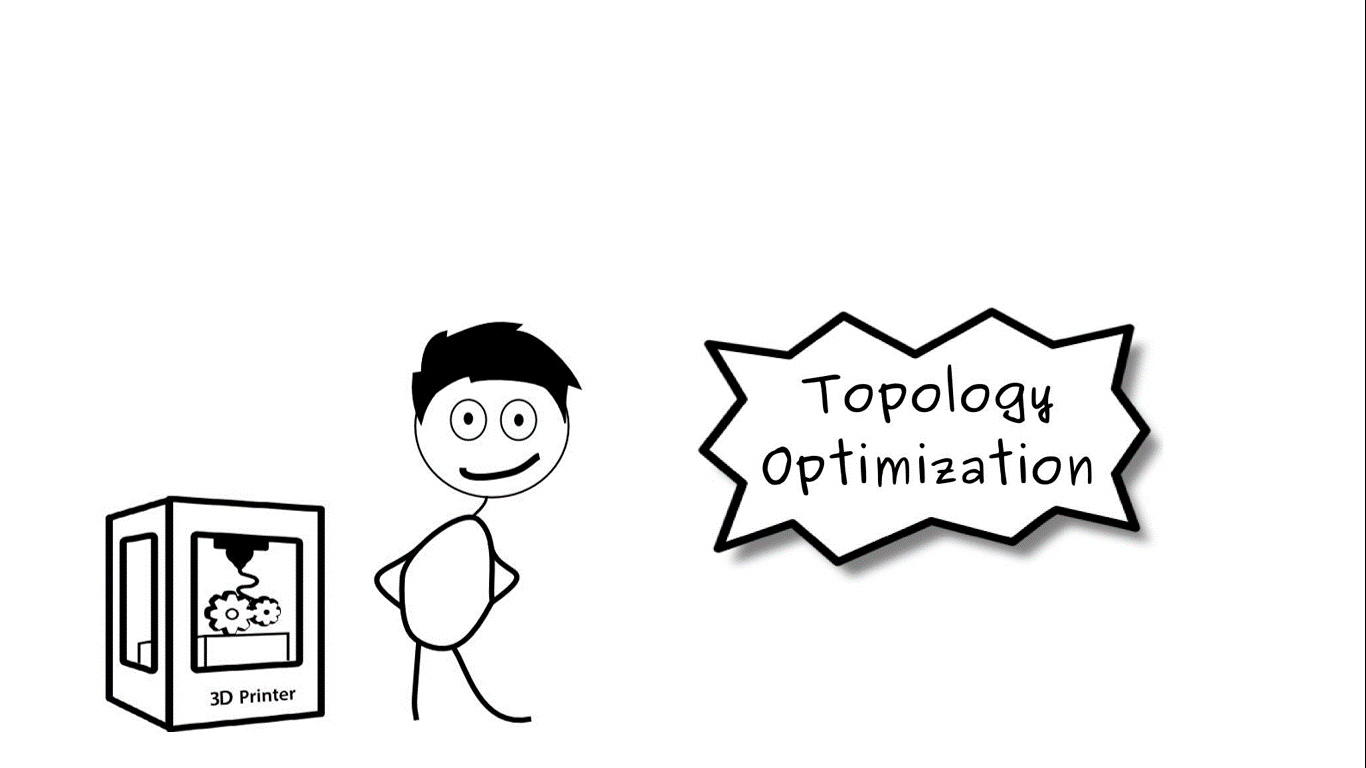
\includegraphics[width=1\linewidth]{Pictures/animations/animation_1.png}
		\end{figure}

\end{frame}

\begin{frame}
\begin{figure}
			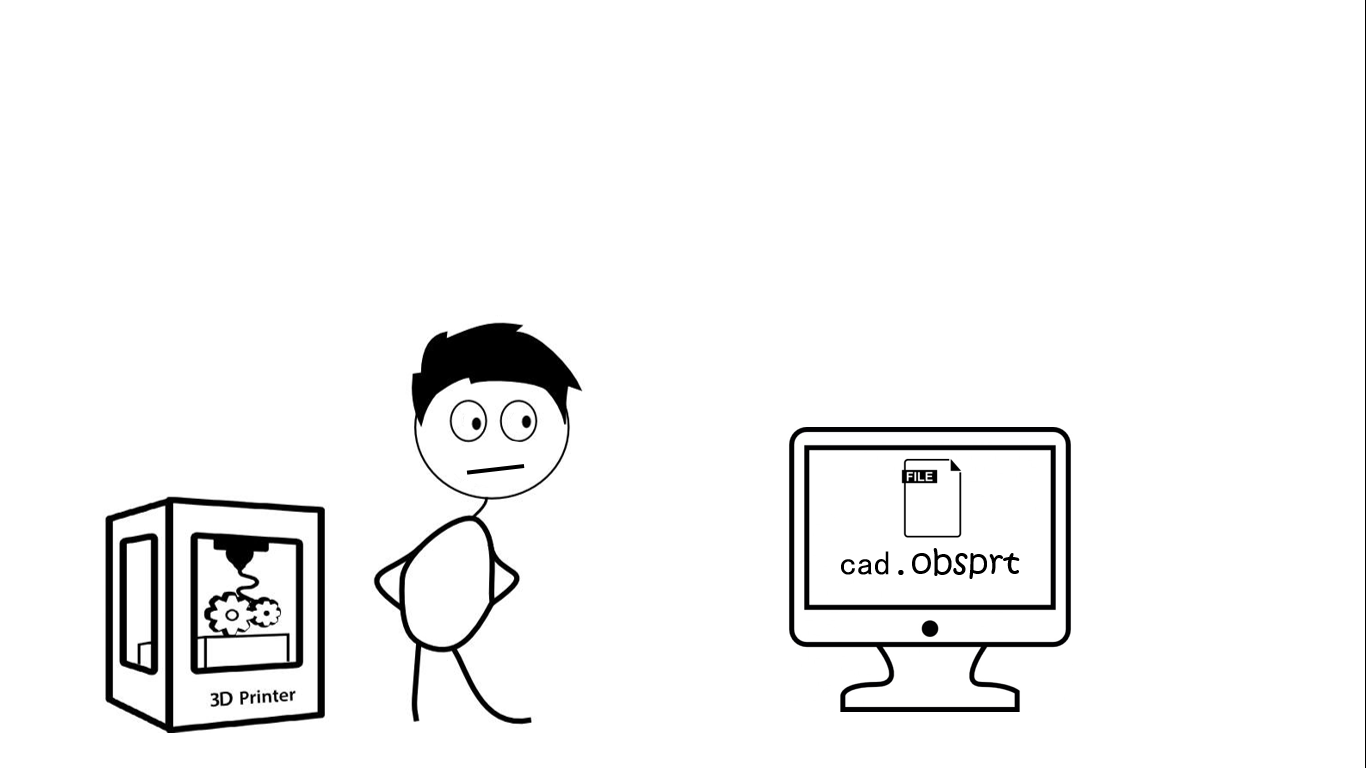
\includegraphics[width=1.4\linewidth]{Pictures/animations/animation_2.png}
		\end{figure}

\end{frame}

\begin{frame}{Design Issues}
	
	
\includegraphics[width=0.175\textwidth, center]{Pictures/animations/animation_designer_sad}
	
	\begin{multicols}{2}
		%\underline{Problem:}
		\setbeamercolor{block}{bg=white,fg=cyan}
		\begin{block}{Problems:}{
		\begin{itemize}		
			\item Engineering-design processes are a pendulum!
			\item Topology-Optimization algorithms are a one-way street!
		\end{itemize}~\\
		}
		%\begin{variableblock}{Focus:}{bg=cyan,fg=white}	
		\end{block}
		\columnbreak

		\begin{block}{Desired:}{
		\begin{itemize}		
			\item[$\Rightarrow$] One-click optimization
		\end{itemize}
		\begin{itemize}		
			\item[$\Rightarrow$] Full-circle optimization process	
		\end{itemize}
		}
		\end{block}
				
		\end{multicols}

\end{frame}	

\begin{frame}{Features}
	
	\begin{block}{Fully integrated design process}{
			\begin{itemize}		
				\item CAD to CAD
				\item Turnkey
				\item Standardized I/O			
			\end{itemize}~\\
		}
	\end{block}
	\begin{block}{Control to the user}{
			\begin{itemize}		
				\item Resolution
				\item Smoothness
				\item Localized Optimization			
			\end{itemize}~\\
		}
	\end{block}	
	\begin{block}{100\% open source}{
			%\begin{itemize}		
			%\end{itemize}~\\
		}
	\end{block}
	
\end{frame}

\begin{frame} {Power to the user}
	
	\begin{block} {Geometry} {
			\begin{itemize}
				\item Original geometry
				\begin{itemize}
					\item[-] Load(s)
					\item[-] Fixture(s)
				\end{itemize}
				\item Modifiable region(s)
				\item Non-modifiable region(s)
			\end{itemize}
			}
	\end{block}
	\pause
	
	\begin{block} {Solution Parameters} {
			\begin{itemize}
				\item Optimization accuracy
				\item Level of surface approximation
				\item Surface smoothness
			\end{itemize}
			}
	\end{block}
		
\end{frame}

\begin{frame}{Features}

\begin{block}{Fully integrated design process}{
		\begin{itemize}		
			\item CAD to CAD
			\item Turnkey
			\item Standardized I/O			
		\end{itemize}~\\
		}
		\end{block}
\pause
\begin{block}{Control to the user}{
		\begin{itemize}		
			\item Resolution
			\item Smoothness
			\item Localized Optimization			
		\end{itemize}~\\
		}
		\end{block}
\pause		
\begin{block}{100\% open source}{
		%\begin{itemize}		
		%\end{itemize}~\\
		}
		\end{block}

\end{frame}
		